\chapter{Языки разработки моделей и~аппаратуры}\label{chapter12}

\dictum[Linus Torvalds]{Talk is cheap. Show me the code.}
 
Поскольку симуляторы и отдельные модели устройств сами по себе являются программами, они пишутся на некотором выбранном языке (или нескольких языках) программирования, как правило, высокого уровня. 

В законченном симуляторном решении, претендующем на право называться удобным и расширяемым, можно выделить функциональные блоки, различные по своему назначению (примерный состав приведён на рис.~\ref{fig:breakdown}). 
\begin{figure}[htb]
    \centering
    % \includegraphics[width=\textwidth]{./breakdown-crop.pdf}
\begin{tikzpicture}[>=latex, font=\small]
    \node[] (gui) {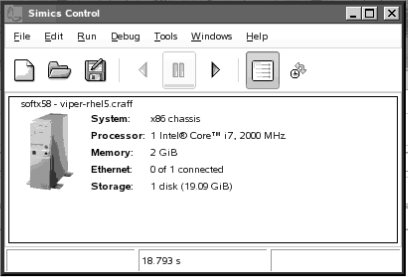
\includegraphics[width=2cm]{./gui.png}};
    \node[above=0.1cm of gui] {Графический интерфейс};
    
    \node[ node distance = 3cm, right of=gui] (device1) {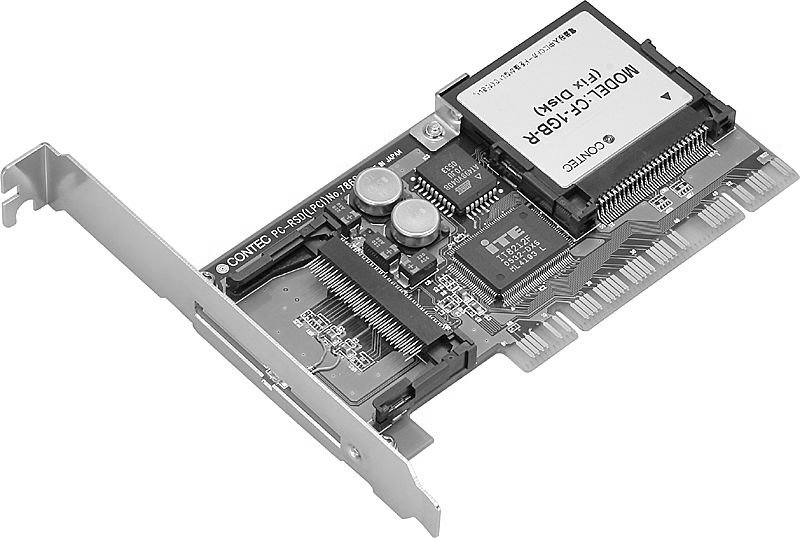
\includegraphics[height=1.5cm]{./device1.png}};
    \node[node distance = 2cm, right of=device1] (device2) {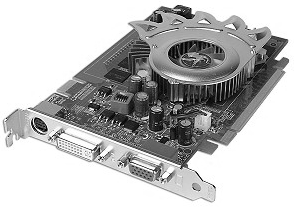
\includegraphics[height=1.5cm]{./device2.png}};
    \node[node distance = 2cm, right of=device2] (device3) {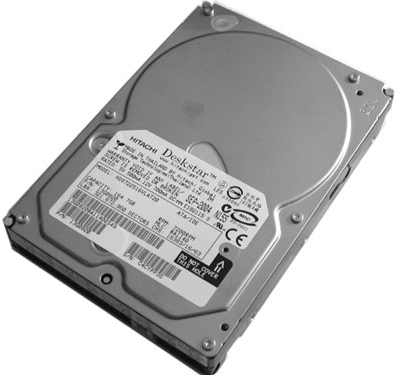
\includegraphics[height=1.5cm]{./device3.png}};
    
    \node[draw, fit=(device1) (device3)] (frame) {};
    
    \node[node distance = 3cm, below of=gui] (cli) {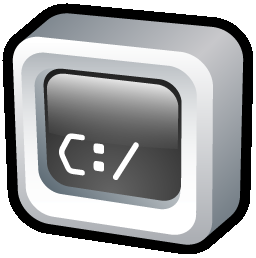
\includegraphics[height=1.5cm]{./cli.png}};
    
    \node[node distance = 3cm, below of=device1] (python) {
\includegraphics[height=1.5cm]{./python.png}};
    \node[node distance = 2cm, right of=python] (perl) {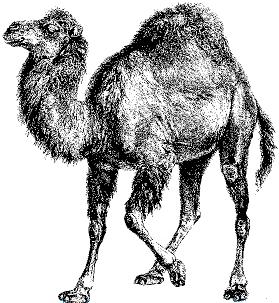
\includegraphics[height=1.5cm]{./perl.png}};
    \node[node distance = 2cm, right of=perl] (lua) {
\includegraphics[height=1.5cm]{./lua.png}};
    
    \node[above=0.1cm of cli] {Командная строка};
    \node[above=0.1cm of perl] {Язык сценариев};
    \node[above=0.1cm of device2] {Модели устройств};
    
    % \draw[<->] (gui.south east) -- (python.north west);
    % \draw[<->] (frame.south west) -- (cli.north east);
    
\end{tikzpicture}
    \caption[Классификация компонент симулятора]{Классификация компонент симулятора. Графический интерфейс и командная строка отвечают за взаимодействие с пользователем, поддержка языков сценариев (скриптов) обеспечивает средства автоматизации и расширения функциональности, модели устройств являются основным вопросом данной главы}
    \label{fig:breakdown}
\end{figure}

При этом каждая подсистема может быть реализована на своём языке, наиболее адекватном требуемой функциональности. Например, графический интерфейс может быть сделан с помощью библиотек (языков) Qt (С++), AWT (Java), Tk (Tcl) и т.д. Интерпретатор сценариев, скорее всего, будет выполнен на том же динамическом языке, который предполагается использовать для написания скриптов.

Перейдём к основной части любого симулятора --- моделям устройств. Для их создания можно использовать языки общего назначения, такие как Си, Си++, и писать весь симулятор и каждую модель «с нуля». Однако специфика создаваемого кода такова, что является возможным выделение некоторых абстракций в законченные модули, удобные для повторного использования, и интеграции моделей, написанных разными людьми, с помощью набора документированных интерфейсов.

По этой причине в индустрии программного моделирования можно выделить два подхода.

\begin{enumerate*}
\item \textit{Создание библиотек для} Си/Си++, \textit{реализующих полезные для  моделирования примитивы.} Желаемые понятия формулируются на языках общего назначения в терминах типов данных и функций или объектов, полей и методов для объектно-ориентированных языков. У разработчика, использующего такую систему, остаётся полная свобода выражения, ограниченная лишь синтаксисом применяемого языка.

\item \textit{Использование специализированных языков описания моделей.} Концепции моделирования вносятся в ядро языка, что уменьшает сложность создаваемых кодов и повышает темп разработки. Однако требуется некоторое время и усилия для того, чтобы разработчики освоили новый язык.
\end{enumerate*}

Схожая задача возникает перед разработчиками аппаратуры --- необходимость иметь способ описания алгоритма работы устройства. При этом для данной задачи языки общего назначения применимы ещё меньше, так как оперируют не теми базовыми абстракциями; поэтому практически всегда используются языки специализированные. Однако здесь преследуется иная цель: получить структуру, из которой возможно генерировать описание физического расположения элементов на кристалле разрабатываемой микросхемы, пригодного для изготовления настоящих экземпляров устройства на фабрике. Генерация симулятора системы также возможна и широко используется на финальных этапах разработки, однако степень детализации симуляции часто превышает необходимую ---  модель получается чрезвычайно медленная. Это, в том числе, ограничивает масштаб модели одной или несколькими микросхемами, тогда как часто требуется симулятор, содержащий в себе весь комплекс целиком.

\section{Разработка моделей}

\subsection{Требования на языки}

Всякий язык высокого уровня призван сделать процесс разработки программ определённого типа менее сложным, чем это представляется при использовании языков данной машины --- ассемблера или даже двоичного машинного кода. Достигается такое упрощение введением некоторых понятий, часто применяемых в программе, и переформулированием их в виде, удобном для человека. Например, в спецификации языка Си можно увидеть такие понятия, как переменная, имеющая имя (в машинном коде есть только безымянные ячейки памяти), типы, логически выстраивающие структуру данных, функции, объединяющие в себе действия, часто совершаемые совместно в фиксированном порядке и т.п. 

Указанный перечень абстракций применим для очень широкого класса создаваемых программ, в том числе и программ-симуляторов аппаратуры. Однако обычно его недостаточно или он неточно ложится в рамки задачи (например, в счётчике импульсов нет переменных, зато есть регистры). Перечислим некоторые дополнительные абстракции, часто встречаемые в аппаратуре, но не в программах общего назначения.

\begin{enumerate*}
\item \textit{Сигналы.} Простейший сигнал --- это логический уровень (единица или ноль), наблюдаемый на одном проводнике. Также сигналом может быть факт изменения (т.н. фронт) с высокого уровня на низкий  или наоборот.

\item \textit{Шины.} За один такт часто требуется передать не один бит информации, а несколько, при этом набор проводников объединяется в логическую группу, например, из 8, 16, 32 однобитных сигналов.

\item \textit{Операции над отдельными битами чисел.} Базовая функциональность присутствует во всех языках общего назначения, но описание функций аппаратуры требует более гибких методов, как то: операции над диапазонами бит, применение масок, сдвиги, числа с длиной, не кратной восьми,  и т.п.

\item \textit{Транзакции} отражают мгновенность акта передачи нескольких сигналов по шине, а также направление сигнала (т.е. отправителя и получателя).

\item \textit{Расширенные значения для уровней сигналов.} Кроме «высокого» и «низкого» значения в реальной аппаратуре, выходы могут быть в т.н. непроводящем (hi-Z) или в неопределённом (Х) состояниях.

\item \textit{Абстракции хранения данных} включают в себя одиночные и группы регистров разной ширины, банки памяти различной ёмкости.

\item \textit{Карты памяти.} Обращение некоторого устройства по адресу в памяти может быть обработано различными устройствами в зависимости от значения адреса; при этом правило определения обработчика может быть сложным или динамически зависеть от сторонних условий.

\item \textit{Побочные эффекты} от обращения к регистрам при чтении и записи. 

\item \textit{Задержки событий.} Симулируемые действия могут иметь различные задержки в симулируемом времени.
\end{enumerate*}

\subsection{SystemC и TLM}

\textbf{SystemC} --- язык проектирования и верификации моделей системного уровня, реализованный в виде библиотеки C++, которая включает компоненты дискретного моделирования событий~\cite{systemc2006}.

SystemC курируется организацией «Open SystemC Initiative», созданной в 1999 году, был принят ассоциацией IEEE как стандарт IEEE 1666-2005, обновленный в 2011 году как IEEE 1666-2011. Существует «эталонная» реализация данной библиотеки, однако большое количество компаний-разработчиков аппаратуры  выпустили свои реализации и инструменты, основанные на спецификации и совместимые между собой.

Язык использует возможности нижележащего С++ для объектной декомпозиции разрабатываемых моделей, а также возможностей шаблонного описания используемых данных. 

Несмотря на то, что первая версия SystemC решала поставленную перед ней задачу адекватного отражения необходимых понятий моделирования, было принято решение об улучшении степени абстрагирования отдельных подкомпонент и транзакций от деталей их реализации. Это расширение было создано согласно принципам \textbf{TLM} (\abbr Transaction Level Modeling)~\cite{tlm2003} и вошло во вторую версию стандарта SystemC. 

Пример кода, использующего SystemC\footnote{Приведённые ниже примеры кода на языках SystemC, Verilog  и VHDL взяты из Wikipedia.}.

\begin{lstlisting}
#include "systemc.h"
SC_MODULE(adder) {        // module (class) declaration
  sc_in<int> a, b;        // ports
  sc_out<int> sum;
  void do_add() {         // process
    sum.write(a.read() + b.read()); //or just sum = a + b
  }
  SC_CTOR(adder) {        // constructor
    SC_METHOD(do_add);    // register do_add to kernel
    sensitive << a << b;  // sensitivity list of do_add
  }
};
\end{lstlisting} 

\subsection{Специализированные языки}

Как уже было сказано во введении к главе, зачастую создаются \textbf{предметно-ориентированные} языки (\abbr domain specific languages), специально предназначенные для разработки аппаратуры. Это рационально при условии, что они используются как часть большого пакета для моделирования систем.

\paragraph{Пример: DML}

Другим примером языка, специально созданного для описания функциональных моделей устройств, является DML (Device Modeling Language), используемый в симуляторе Simics~\cite{dml-tutorial}, в котором упор сделан на максимально быстрое модельное прототипирование устройств, т.е. создание заготовки устройства, не имеющей полной функциональности, но предоставляющей все внешние интерфейсы реального устройства. Этот подход позволяет реализовывать сложные системы постепенно, притом концентрироваться на самых  важных функциональных аспектах в первую очередь и дописывать недостающие компоненты после. Основной тип устройств, описываемых с помощью DML, --- это неисполняющие устройства, он не используется для создания моделей процессоров.

Синтаксис DML предоставляет программисту конструкции для описания банков регистров, интерфейсов и функционального поведения устройств. Использование DML для написания модели автоматически гарантирует многие декларируемые Simics свойства у получаемых моделей.

\begin{itemize*}
\item Явное представление архитектурного состояния в \textit{атрибутах}.
\item Корректное сохранение и загрузка состояния симуляции из точек сохранения.
\item Безопасная многопоточность (\abbr thread safety).
\item Поддержка правильного порядка байт данных (т.н. Endianness) при взаимодействии моделей между собой.
\item Генерация текста документации из комментариев и строк описания деталей модели.
\end{itemize*}

Существующий компилятор \texttt{DMLC} является т.н. source-to-source компилятором, т.е. результатом его работы являются не машинные инструкции, а промежуточный текст на языке Си, который затем обрабатывается компилятором GCC. Однако при этом двухстадийном процессе сохраняется отладочная информация о строках исходного DML-кода, что позволяет использовать специально модифицированный вариант отладчика GDB, «понимающего» синтаксис DML для работы с исходным, а не с промежуточным кодом при отладке. Дополнительно этот подход позволяет при необходимости с помощью специальных команд языка включать код на Си в программу на DML, при этом такие куски передаются в промежуточный код без изменений.

\textbf{Пример кода на DML} % dammit I don't know why \paragraph does not work.

\begin{lstlisting}
register lcr { 
  parameter soft_reset_value = 0x00; 
  parameter hard_reset_value = 0x00; 
  field wls          [1:0] "Word length select "; 
  field stb          [2] "Number of stop bits (0 = 1, 1 = 2)"; 
  field pen          [3] "Parity enable (0 = disable, 1 = enable)"; 
  field eps          [4] "Even parity select (0=Odd, 1=Even)"; 
  field stick_parity [5] "Stick parity"; 
  field set_break    [6] "Set break"; 
  field dlab         [7] "Divisor latch access bit"; 
  // After a write to this register, check the contents of WLS and  
  // set the character length mask appropriately 
  method after_write (memop) { 
    if      ($wls == 0) $mask = 0x1F; 
    else if ($wls == 1) $mask = 0x3F; 
    else if ($wls == 2) $mask = 0x7F; 
    else                $mask = 0xFF; 
  } 
}   
\end{lstlisting} 


\subsection{Языки описания набора инструкций}

Отдельное внимание следует уделить разработке моделей процессоров и языкам, предназначенным для их создания.

Сложность данной задачи заключается в том, что при разработке совершенно нового устройства его авторам требуется иметь в рабочем состоянии одновременно  несколько инструментов и документов из следующего списка:

\begin{itemize*}
\item функциональный симулятор набора инструкций;
\item точная потактовая модель;
\item дизассемблер машинного кода;
\item компилятор с языка высокого уровня в машинный код;
\item документация к аппаратуре;
\item иногда необходимо также уметь генерировать синтезируемое описание новой архитектуры.
\end{itemize*}

Если каждая компонента разрабатывается отдельно, то при изменении спецификации процессора (что происходит часто на ранних этапах исследования) приходится вносить изменения во всех программах и документах, что чревато ошибками и десинхронизацией инструментов, каждый из которых фактически имеет собственный «взгляд» на одно и то же устройство.  

Существует несколько проектов языков, призванных решить всю описанную задачу. В качестве примера см. LISA~\cite{wahlen2004c,zivojnovic1996,schliebusch2002}, ISDL~\cite{Hadjiyiannis97isdl:an,isdl1997} и~\cite{hoffmann2001}. Решение состоит в автоматической генерации необходимых инструментов из одного описания (рис.~\ref{fig:lisa}). 

\begin{figure}[htb]
    \centering
%     \includegraphics[width=0.5\textwidth]{./lisa-crop.pdf}
\begin{tikzpicture}[>=latex, font=\small]
\def\gear{
    \begin{tikzpicture}
    \draw[scale=1]
    \foreach \i in {1,2,...,10} {% draw the gear
        [rotate=(\i-1)*36]  (0:0.5)  arc (0:12:0.5) -- (18:0.7)  arc (18:30:0.7) --  (36:0.5)
    };
    \end{tikzpicture}
}
    \node[draw, tape] (src) {Исходное описание}
    [level distance=2cm, sibling distance=2.5cm, edge from parent/.style={draw, ->}]
    child {node[] {\gear}
        child {node {Дизассемблер}}
    }
    child {node[] {\gear}
        child {node {Симулятор}}
    }
    child {node[] {\gear}
        child {node {Документация}}
    };
\end{tikzpicture}
    \caption{Генерация инструментов разработки из общего описания архитектуры}
    \label{fig:lisa}
\end{figure}


Одним из недостатков этого подхода является зачастую субоптимальная скорость или качество работы получаемых инструментов; например, компилятор может генерировать не самый быстрый или компактный код, функциональная модель работает медленнее, чем могла бы будучи написанной человеком, синтезируемое описание занимает излишне много места на кристалле и т.д. Тем не менее скорость создания, модификации и степень согласованности всех инструментов часто перевешивают эти огрехи на ранних этапах, а затем, после фиксации спецификаций, все инструменты могут быть переписаны «вручную», с необходимыми оптимизациями.

Другой аспект, возникающий при создании моделей процессоров --- желание иметь её с более чем одним механизмом симуляции, например, создать интерпретатор и двоичный транслятор и затем иметь возможность переключаться между ними. И снова для того, чтобы избежать рассинхронизации суб-моделей при правках спецификаций, чаще всего избирается подход,  при котором они генерируются из одного описания семантики инструкций~\cite{simgen}.

Для построения двоичных трансляторов также может использоваться преобразование описаний семантики гостевых инструкций в заготовки машинного кода, при этом исходное описание является неким метаассемблером, преобразуемым в настоящий ассемблер хозяйской архитектуры (рис.~\ref{fig:capsules}). Такой подход позволяет разработчику иметь наибольший контроль над создаваемым двоичным транслятором~\cite{MyConfMIPT52}. Существенным недостатком является полная непереносимость модели на другую хозяйскую архитектуру, т.к. при этом приходится переписывать весь код эмуляции инструкций.

\begin{figure}[htb]
    \centering
%     \includegraphics[width=0.75\textwidth]{./capsules-crop.pdf}
\begin{tikzpicture}[>=latex, font=\small]
\def\gear{
    \begin{tikzpicture}
    \draw[scale=1]
    \foreach \i in {1,2,...,10} {% draw the gear
        [rotate=(\i-1)*36]  (0:0.5)  arc (0:12:0.5) -- (18:0.7)  arc (18:30:0.7) --  (36:0.5)
    };
    \end{tikzpicture}
}
\node[draw, tape, text width=9cm, align=left, font=\footnotesize\ttfamily] (src){
NJU(U32 @Curr_IP, U32 @op_size, X128 @ireg_dst)\\
\{\\
@UPDATE_Curr_IP(@Curr_IP)\\
\ \ \ \ movl  \$@op_size,  @glst_arg0_w0(\%ebp)\\
\ \ \ \ cmpss \$0xffff, (\%esi), @ireg_dst\\
\}\\
};

\node[above=0.15cm of src] {Исходное описание};

\node[below=0.5cm of src] (gear) {\gear};

\node[minimum height=1.8cm, inner sep=2pt, below=0.5cm of gear, xshift=-3cm, draw, tape, text width=4cm, align=left, font=\scriptsize\ttfamily] (asm){
movl  \$0xdeadc0de,  12(\%ebp) \\
cmpss \$0xffff, (\%esi), \%ebx \\
};

\node[below=0.15cm of asm] {Ассемблер};

\node[minimum height=1.8cm, inner sep=2pt, below=0.5cm of gear, xshift=3cm, draw, tape, text width=4.5cm, align=left, font=\scriptsize\ttfamily] (emitter){
\#define NJU\textbackslash\\
(Curr_IP, op_size, ireg_dst)\textbackslash \\
...
};
\node[below=0.15cm of emitter] {Эмиттер};

\draw[->] (src) -- (gear);
\draw[->] (gear) -- (asm);
\draw[->] (gear) -- (emitter);
\end{tikzpicture}
    \caption[Создание двоичного транслятора из метаассемблера]{Создание двоичного транслятора из метаассемблера. Исходное описание содержит в себе аргументы создаваемой функции и ассемблерные инструкции хозяйской архитектуры. После процесса обработки мы имеем два блока исходного кода --- ассемблерный код, используемый при симуляции, а также код на Си (эмиттер), передающий первому аргументы на этапе трансляции}
    \label{fig:capsules}
\end{figure}


\section{Языки разработки аппаратуры}


В заключение кратко познакомимся с двумя самыми популярными языками описания аппаратуры (\abbr Hardware Definition Language, HDL), используемыми в настоящее время --- Verilog и VHDL.

\subsection{Verilog}
 
Verilog был создан Филом Мурби и Прахбу Гоелом в  1984 году в фирме Auto\-mated In\-te\-gra\-ted De\-sign Sys\-tems. Он был принят как стандарт IEEE 1364-1995. Позже дополнения к языку Verilog-95 были приняты как IEEE 1364-2001 (или Veri\-log-2001). Следующий вариант, Verilog 2005 (стандарт IEEE 1364-2005), добавил небольшие исправления, уточнения спецификаций и несколько новых синтаксических конструкций.

Разработчики Verilog сделали его синтаксис очень похожим на синтаксис языка C, что упрощает освоение. Язык имеет препроцессор, очень похожий на препроцессор языка C, и основные управляющие конструкции \texttt{«if»}, \texttt{«while»} также подобны одноимённым конструкциям языка C. 

Существует подмножество инструкций языка Verilog, называемое синтезируемым. Модули, которые написаны на этом подмножестве, называют \textbf{RTL} (\abbr register transfer level --- уровень регистровых передач). Они могут быть физически реализованы с использованием САПР-синтеза. Данные САПР по определённым алгоритмам преобразуют абстрактный исходный код на Verilog в netlist --- логически эквивалентное описание, состоящее из элементарных логических примитивов (например, AND, OR, NOT, триггеры), которые доступны в выбранной технологии производства СБИС или программирования БМК и ПЛИС. Дальнейшая обработка netlist в конечном итоге порождает фотошаблоны для литографии или прошивку для FPGA.

Что отличает этот язык от обычных языков общего назначения? Во-первых, разделение всех команд на \textbf{синтезируемые}, т.е. непосредственно представляемые в аппаратуре, и на \textbf{несинтезируемые}, используемые только для отладки и симуляции.

Оператор \texttt{<=} в Verilog является ещё одной особенностью языка описания аппаратных средств, отличающей его от процедурных языков общего назначения. Сама операция известна как \textit{неблокирующее присваивание}. Применение оператора не имеет внешне видимого эффекта до наступления следующего такта. Это означает, что порядок таких присваиваний в коде не может влиять на суммарный эффект функции, т.к. все они произойдут одновременно и произведут тот же результат: значения \texttt{flop1} и \texttt{flop2} будут обмениваться значениями на каждом такте.

Другой оператор присваивания, <<\texttt{=}>>, является блокирующим. Когда он используется, переменная с его левой стороны обновляется немедленно. В приведённом выше примере, если бы использовался <<\texttt{=}>> вместо <<\texttt{<=}>>, \texttt{flop1} и \texttt{flop2} не обменялись бы значениями. Вместо того, как и в традиционном процедурном программировании, компилятор воспринял бы это как указание сделать их содержимое одинаковым.

\textbf{Пример кода на Verilog: триггер} % dammit I don't know why \paragraph does not work.

\begin{lstlisting}
module toplevel(clock,reset);
 input clock;
 input reset;
 reg flop1;
 reg flop2;
 always @ (posedge reset or posedge clock)
 if (reset)
   begin
     flop1 <= 0;
     flop2 <= 1;
   end
 else
   begin
     flop1 <= flop2;
     flop2 <= flop1;
   end
endmodule         
\end{lstlisting}

\subsection{VHDL}

VHDL был разработан в 1983 г. по заказу Министерства обороны США с целью формального описания логических схем для всех этапов разработки электронных систем, начиная с модулей микросхем и заканчивая крупными вычислительными системами.

Первоначально язык предназначался для моделирования, но позднее из него было выделено синтезируемое подмножество. Средствами языка VHDL возможно проектирование на различных уровнях абстракции (поведенческом или алгоритмическом, регистровых передач, структурном) в соответствии с техническим заданием и предпочтениями разработчика. Представляется возможным выделить следующие три составные части языка: алгоритмическую, основанную на языках Ada и Pascal и придающую языку VHDL свойства процедурных языков, и проблемно ориентированную, обращающую VHDL в язык описания аппаратуры, а также объектно-ориентированную, интенсивно развиваемую в последнее время.

\textbf{Пример кода на VHDL} % dammit I don't know why \paragraph does not work.

\begin{lstlisting}
-- latch template 1:
Q <= D when Enable = '1' else Q;
-- latch template 2:
process(D,Enable)
begin
  if Enable = '1' then
    Q <= D;
  end if;
end process;
\end{lstlisting} 

\iftoggle{hasquiz}{
    \section{\Questions к главе \ref{chapter12}} %\label{chapter12-questions}

\subsection*{Вариант 1}

\begin{questions}

\question[3] Какое утверждение наилучшим образом характеризует термин SystemC?
\begin{choices}
    \choice Компилятор языка Си с дополнениями для моделирования систем.
    \choice Язык программирования, похожий на Си.
    \choice Язык программирования, похожий на С++.
    \correctchoice Набор библиотек для С++.
\end{choices}

\question[3] Язык DML используется для разработки
\begin{choices}
    \correctchoice функциональных моделей,
    \choice потактовых моделей,
    \choice гибридных моделей.
\end{choices}

\question[3] Текущая реавлизация комилятора DMLC является
\begin{choices}
    \choice компилятором типа source-to-source с промежуточным языком С++,
    \choice компилятором, преобразующим исходный текст в байткод Java,
    \correctchoice компилятором типа source-to-source с промежуточным языком Си,
    \choice классическим компилятором,
    \choice частичным интерпретатором.
\end{choices}

\question[3] Закончите фразу: Языки разработки аппаратуры
\begin{choices}
\choice не используются для начального моделирования устройств, так как могут быть преобразованы только в netlist,
\correctchoice не используются для начального моделирования устройств, так как получаемые модели очень медленны,
\choice не используются для начального моделирования устройств, так как могут содержать в себе синтезируюмую часть,
\choice используются для начального моделирования устройств.
\end{choices}

\end{questions}

\subsection*{Вариант 2}

\begin{questions}

\question[3] Какое утверждение наилучшим образом характеризует термин TLM?
\begin{choices}
    \choice Язык программирования, похожий на Си.
    \choice Язык программирования, похожий на С++.
    \choice Среда исполнения моделей DES.
    \correctchoice Расширение стандарта SystemC.
\end{choices}

\question[3] Язык DML используется для разработки
\begin{choices}
    \correctchoice неисполняющих моделей,
    \choice исполняющих моделей,
    \choice как исполняющих, так и неисполняющих моделей.
\end{choices}

\question[3] Какой способ наиболее удобен и надёжен для поддержания набора инструментов моделирования в синхронизированном состоянии при постоянном изменении входной спецификации процессора?
\begin{choices}
    \correctchoice Генерация всех инструментов из единого описания.
    \choice Тщательное сравнение всех инструментов после каждого изменения одного из них.
    \choice Создание одного инструмента, поддерживающего максимальное количество функций.
\end{choices}

\question[3] Закончите фразу: Синтезируемое подмножество языков разработки аппаратуры
\begin{choices}
\choice не может быть использовано для создания netlist и RTL-описаний,
\choice используется только для отладки моделей,
\correctchoice  используется для создания netlist и RTL-описаний.
\end{choices}

\end{questions}

% К каждой лекции должно быть от 8 до 12 задач, у каждой задачи должно быть 3-5 вариантов формулировок примерно одинаковой сложности. Допускается объединение нескольких последовательных лекций в одну тему и подготовка тестов к темам.
% Задачи должны полностью соответствовать материалам лекций, то есть лекциях должно быть достаточно информации для ответа на все вопросы.
% Формулировка каждого варианта задачи должна содержать всю необходимую информацию и не должна ссылаться на тексты внутри лекции, картинки или другие задачи или варианты задачи.
% Правильные ответы выделяются знаком «+» перед их формулировкой. Правильных ответов может быть несколько. Для тестов с несколькими ответами как минимум один ответ должен быть правильным и как минимум один ответ должен быть неправильным. 
% 
% Структура теста к лекции
% 
% \subsection*{Задача 1}
% 
% \paragraph{Вариант 1} 
% 
%     Чему равно 2+2?
%         Ответ 1. 3
%         + Ответ 2. 4
%         …
%         Ответ N. 5
% \paragraph{Вариант 2}
%     Чему равно 2*2?
%         + Ответ 1. 4
%         + Ответ 2. 2+2
%         …
%         Ответ N. 5
% \paragraph{Вариант 3}
% 
%     Чему равно 2-2?
%         Ответ 1. 0
% 
% 
%         
% \section{Просто подборка вопросов}
% 
}{}

\iftoggle{webpaper}{
    \printbibliography[title={Литература}]
}{}


